% you need to build with xelatex
\documentclass[t,aspectratio=169]{beamer}

\usepackage[backgroundTheme=LSST2017-nologos,
  fonts=false, colorlinks=false,
 footline={DM All Hands $\bullet$ IPAC  $\bullet$ March 6--8, 2018},
meeting={DM All Hands},
position={DM Project Manager}
]{LSST-beamer}




\author{William O'Mullane}
\institute{AURA/Rubin Observatory}
\title{LSST Data Management }
\date{  \today}


\graphicspath{ {./images/} {./ETCcharts/} }

\def\pasp{PASP}

\usepackage{pdfpages}
\usepackage{amsmath,graphicx,marvosym}
\usepackage{tikz,multirow,array,colortbl,multimedia}
\usepackage{times,layouts}
\usepackage{tikz,hyperref}
\usetikzlibrary{positioning,arrows,shapes,decorations.shapes,shapes.arrows}
\usetikzlibrary{backgrounds,calc, shadows}
\usetikzlibrary{shapes.callouts}

\usepackage{graphicx}
\usepackage{natbib}
\usepackage{longtable}

\tikzstyle{flow}=[->, >=stealth', thick, shorten >=3pt, shorten <=3pt]

\def\aaps{A\&AS}           % Astronomy and Astrophysics Suplement
\def\aap{A\&A}             % Astronomy and Astrophysics
\def\ssr{Space~Sci.~Rev.}  % Space Science Reviews
\def\apj{ApJ}              % Astrophysical Journal
\def\aj{AJ}                % Astronomical Journal
\def\mnras{MNRAS}          % Monthly Notices of the RAS
\def\araa{ARA\&A}          % Annual Review of Astron and Astrophys
\def\nat{Nature}           % Nature
\def\apjl{ApJ}             % Astrophysical Journal, Letters

\def\degr{\hbox{$^\circ$}}
\def\arcmin{\hbox{$^\prime$}}
\def\arcsec{\hbox{$^{\prime\prime}$}}
\def\fs{\hbox{$.\!\!^{\rm s}$}}
\def\fdg{\hbox{$.\!\!^\circ$}}
\def\farcm{\hbox{$.\mkern-4mu^\prime$}}
\def\farcs{\hbox{$.\!\!^{\prime\prime}$}}
\def\sun{\hbox{$\odot$}}


%\newcommand{\bfvec}[1]{\mbox{$\bf#1$}}
%\newcommand{\citell}{\citeyear}
\newcommand{\citeds}{\citeyear}
%\newcommand{\citellp}{\citeyearpar}
%\newcommand{\citedsp}{\citeyearpar}
\providecommand{\secref}[1]{Section~\ref{#1}}
\providecommand{\appref}[1]{Appendix~\ref{#1}}
\providecommand{\partref}[1]{Part~\ref{#1}}
\providecommand{\tabref}[1]{Table~\ref{#1}}
\providecommand{\figref}[1]{Figure~\ref{#1}}
\providecommand{\eqnref}[1]{Eq.~\ref{#1}}
\providecommand{\reqref}[1]{Req.~\ref{#1}}
\providecommand{\actref}[1]{AI~\ref{#1}}


\newcommand{\jira}[1]{\href{https://jira.lsstcorp.org/browse/#1}{#1}}


\author{William O'Mullane}
\institute{AURA/LSST}
\title{LSST Data Management Status  }
\date{ 6$^{th}$ March 2018}


\graphicspath{{./figures} {./images/}{../../dm-docs/images/} }



\begin{document}

\maketitle
\section{Data Management Overview}

\frame {\frametitle{Organization}
\vspace{-0.6cm}
\begin{columns}
\column{0.7\textwidth}
\begin{center}
      \includegraphics[width=1.0\textwidth]{images/DmOrg}\\
\end{center}
\column{0.3\textwidth}

\vspace{0.1cm}

Welcome Leanne Guy  and thanks to Mario (who stays with us)!!\\
\vspace{0.2cm}
Welcome Michelle Butler  and thanks to  Don\\
\vspace{0.2cm}
Welcome Gabriele Comoretto.\\
\vspace{0.2cm}
Deputies John Swinbank (PM), Colin Slater (PS)  and Yusra AlSayyad (Pipelines)\\
\vspace{0.2cm}
{\color{red} Toughest thing in any project is communication.}
\end{columns}
}


%\frame  {\frametitle{DM Document Tree}
%\begin{center}
% \includegraphics[width=0.8\textwidth]{images/DocTree}
%\end{center}
%}

\frame{\frametitle{Verification is a Priority}
\begin{columns}
\column{0.70\textwidth}
 \includegraphics[width=1.0\textwidth]{images/DMMasterSchedule}
\column{0.30\textwidth}
\\
\vspace {-5.9cm}
Across all of LSST verification is a big topic right now.\\
\vspace {0.5cm}
DM is adopting a test driven schedule to better address this.\\
\vspace {0.5cm}
{\color{red} \citeds{LDM-503} Now generated from P6}
\end{columns}
}

\frame{\frametitle{Verification and Validation}
\textbf{Verification}: Have we built everything we are supposed to build?
\begin{itemize}
\item In line with the Project's System Engineering approach
\item Demonstrate that we cover all requirements on DM
\item \citeds{LDM-503} shows the DM verification matrix
\end{itemize}
\textbf{Validation}: Have we built the right thing and does it work as expected?
\begin{itemize}
\item Must tackle \textit{both} Scientific \textit{and} Operational Validation
\item Talking with with Commissioning Team: some \textit{rehearsals} will be joint
\end{itemize}

\begin{center}
\textbf{\citeds{LDM-503}} addresses DM's plans for verification \& validation.
\end{center}
}



\frame{\frametitle{ High level status }
\begin{itemize}
\item The DM Basline is now the reviewed plan (LCRs processed)
\item S18 detail plans submitted
\item Milestones inow being reported monthly
\item Level 2 milestones achieve in  December
\begin{itemize}
\item LDM-503-2   Test report: HSC Reprocessing -DMTR-51
\item LDM-503-3   Test report: Alert Generation Validation -DMTR-53

\end{itemize}
\item Level 2 milestones delayed  in  December
\begin{itemize}
\item LDM-503-1   Test report: Science Platform with WISE data in PDAC

\begin{itemize}
\item Instability PDAC hardware lack of personnel,
\item Testing commend last week
\end{itemize}
\end{itemize}

\end{itemize}
}


\frame { \frametitle{ High Level Goals }
 \begin{itemize}
   \item{2017: Prototyping data access and first access to hardware}
      \begin{itemize}
        \item{Jun: Prototype Data Access Center with SDSS + WISE Data}
        \item{Aug: Working with camera test stand data}
        \item{Dec: Prototype notebooks, private databases for Science Platform}
     \end{itemize}

   \item{2018: Prototypes for various processes and databases - ``Minimum Viable System''}

     \begin{itemize}
       \item{Jun: Calibration Products accessible through Butler}
       \item{Aug: Mountain base network up}
       \item{Oct: Spectrograph data acquisition}
       \item{Dec: Prototype QA/Commissioning Environment}
     \end{itemize}

   \item{Dec 2019: ComCam L1, L2 Production}
   \item{Dec 2019: Base Center Integration Complete}
   \item{Jun 2020: Camera L1, L2 Production}
   \item{Jul 2021: US Data Access Center Integrated}
 \end{itemize}
 \begin{center}
 \textit{Test plans to confirm milestone completion are under development.}
 \end{center}
}

\frame{\frametitle{Commissioning Start Requirements}

November 2019: DM for Commissioning (minimum required for start of commissioning with ComCam):
\hfill {\bf (See \citeds{LSE-79} \S 3.3 and table 8)}
\begin{itemize}
\item Pipeline: single-frame measurement including ISR, ghost masking, cosmic ray detection, PSF estimation, astrometric and photometric calibration, background estimation, single-frame deblending, master calibration image generation, atmospheric characterization
\item Services: archiving, EFD transformation, Data Backbone for files (Base/NCSA), telemetry gateway, OCS-controlled batch, offline processing
\item LSST Science Platform on Commissioning Cluster: Notebook Aspect, image access, user file storage, batch computing
\end{itemize}
\textbf{Milestones:}
\begin{itemize}
\item LDM-503-9\phantom{0} -- 2018-11-30: on the right track with beta software.
\item LDM-503-11 -- 2019-10-31: verification of ComCam commissioning requirements.

\end{itemize}
}


\frame{\frametitle{ Auxiliary Telescope (AuxTel) }
{\color{red} Before commissioning starts !!!}
\begin{itemize}
\item Auxiliary Telescope should be in Chile by the end of the year.
\item Taking and processing data end 2018 !
\end{itemize}
}


\section{Risks and Opportunities}

\frame{\frametitle{Realized Risks}

As part of the replan  three risks  were realized:

\begin{description}

  \item[DM-062]{Programming team productivity below estimate due to geographical distribution/competing priorities.}
  \item[DM-085]{SUI workload underestimated.}
  \item[DM-087]{SUI requirements change.}

\end{description}

These risks are being addressed in the new DM plan and the associated request to draw on contingency.\\
New management and organization allowed us to reduce exposure on some other risks. \\

This plus assessment of exposure on other risks reduced our risk exposure at the level of $\sim$\$12M (to $\sim$\$12M).


}

\frame{\frametitle{Top risks}

\begin{description}
\item[DM-018]{Computing power required for Data Release Production exceeds estimates
\begin{itemize}
	\item Lots of verification testing (e.g. HSC processing)
\end{itemize}
}

\item[DM-023]{Unanticipated characteristics of real data result in poor MultiFit performance (computational)
\begin{itemize}
	\item Lots of verification testing (e.g. HSC processing)
\end{itemize}
}

\item[DM-042]{Loss of key personnel
\begin{itemize}
    \item{Management structure reducing `single points of failure'}
    \item{Focus on written design documentation \& verification plans}
\end{itemize}
}

\item[DM-021]{ Object counts exceed expectations, leading to insufficient compute
\begin{itemize}
\item Improved modeling: work in progress (Juri\'c)
\end{itemize}
}

\item[DM-032]{LSST DM hardware architecture becomes antiquated
\begin{itemize}
	\item{Core algorithmic code is flexible and hardware-agnostic}
    \item{Actively tracking and anticipating the state of the art}
\end{itemize}
}
\end{description}
}

\section{Status }
\frame{\frametitle{Architecture Accomplishments}
\begin{itemize}
\item Requirements and Tests
	\begin{itemize}
		\item DM system requirements (LSE-61) update and verification matrix
		\item Butler Working Group: use cases (LDM-592) and requirements (LDM-556)
		\item TCS interface (LSE-75) revision
		\item Early Integration Activity definitions and organization
		\item Input to Special Programs constraints (DMTN-065)
		\item Experiment with Microsoft, JHU and new SQL Server (PLATO)
	\end{itemize}
\item Design
	\begin{itemize}
		\item LDM-148 system design and LDM-294 product tree update
		\item LDF design and interface refinement as input to LDF ITC design document (LDM-129)
		\item Header Service and middleware design reviews
	\end{itemize}
\item Implementation
	\begin{itemize}
		\item Butler Gen3 implementation
		\item Python: pytest, removal of Py2-only code, flake8
		\item Requirements verification tool prototype
	\end{itemize}
\end{itemize}

}

\frame{\frametitle{Architecture Plans}
\begin{itemize}
\item Requirements and Tests
	\begin{itemize}
		\item ICDs: OCS (LSE-72), DAQ (LSE-68), EPO (LSE-131)
		\item DM Test Plan (LDM-503) milestone definitions
	\end{itemize}
\item Design
	\begin{itemize}
		\item Middleware design document (LDM-152) update
		\item Rethink release processes, packaging, distribution
	\end{itemize}
\item Implementation
	\begin{itemize}
		\item Butler Gen3 implementation
		\item Requirements verification tool
		\item TAP/ADQL queries for IVOA
	\end{itemize}
\end{itemize}

}

\begin{frame}{Alert Production: Recent achievements}

\begin{itemize}
\item{\texttt{SkyWcs}}
\item{Jointcal: replacing meas\_mosaic}
\item{Alert distribution system: benchmarking \& technology}
\item{End-to-end pipeline, incl. LDM-503-3}
\item{Stack DCR}
\end{itemize}

\end{frame}

\begin{frame}{Data Release Production}

\only<1-2>{
\textbf{LDM-503-2: HSC reprocessing milestone}

\begin{itemize}

  \item{First (equal) post-replan, NSF-visible milestone hit by the project.}
  \item{Joint effort to reprocess (LDF team) and analyze (DRP team) HSC data
  under operations-like conditions}
  \item{Milestone successful!}

\end{itemize}
}

\invisible<1>{
  \textbf{``Warp Compare'' coadds}

  \begin{itemize}
    \item{New algorithm to robustly reject artefacts when coadding images.}
    \item{Now default for HSC processing; stack-wide default to be RFCed soon.}
  \end{itemize}

  \begin{center}
  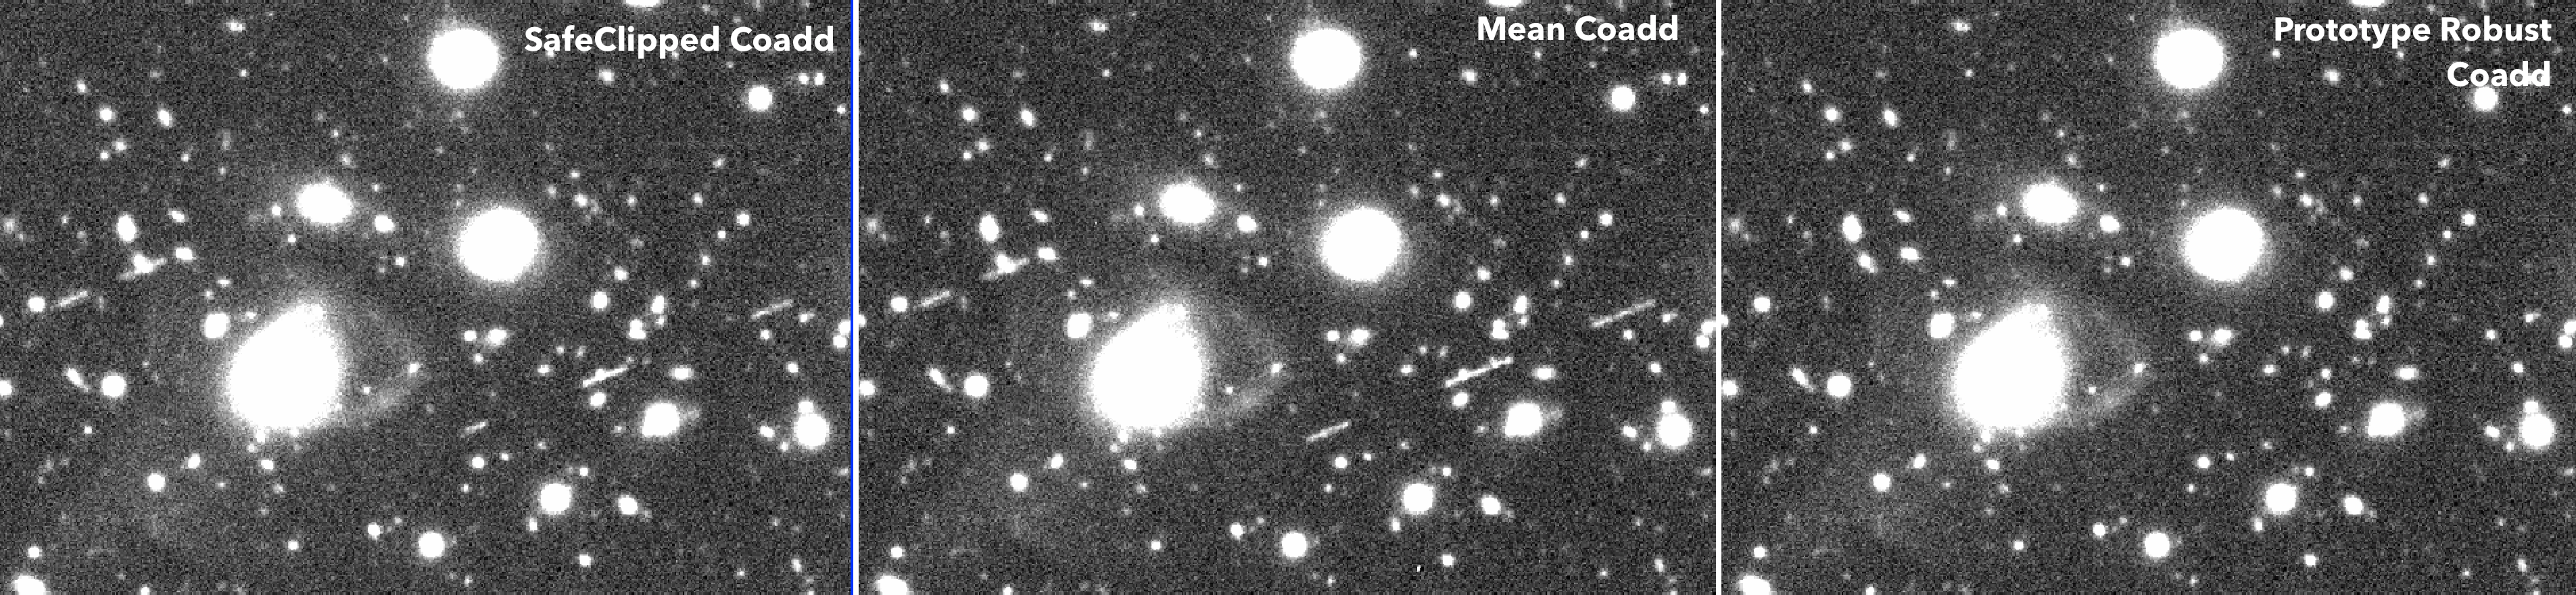
\includegraphics[width=0.5\textwidth]{figures/warpcompare.png}\\
  \tiny Figure: AlSayyad.
  \end{center}
}

\end{frame}

\begin{frame}{Data Release Production}

\textbf{Scarlet: the ``new deblender''}

\begin{itemize}
 \only<1-2>{\item{Key pipeline component; separates overlapping astrophysical objects
 into their constitutent components for measurement.}
  \item{Recent activities:
    \begin{itemize}
      \item{Prototype code developed over the last $\sim$year with exceptionally
      promising results.}
      \item{Journal paper describing the algorithm submitted.}
    \end{itemize}
  }}
  \invisible<1>{\item{Coming up:
    \begin{itemize}
      \item{Performance optimization.}
      \item{Demonstrate performance at-scale on real data with real
      pathologies.}
      \item{Considering how deblender results should affect our approach to
      measurement.}
    \end{itemize}
  }}
\end{itemize}

\begin{center}
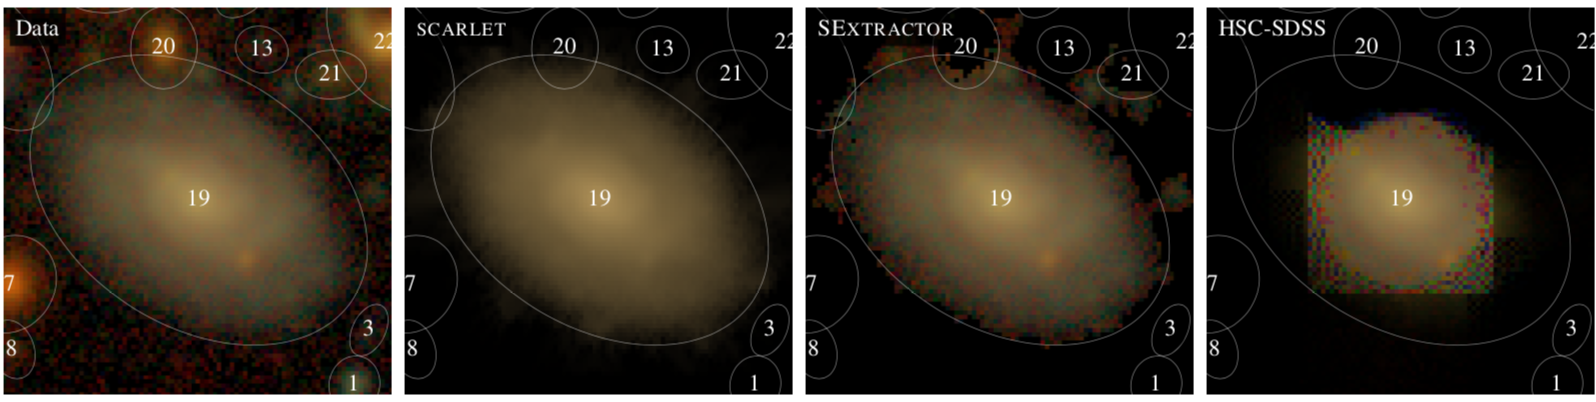
\includegraphics[width=0.5\textwidth]{figures/scarlet.png}\\
\tiny Figure: Melchior et al., 2018
\end{center}

\end{frame}

\begin{frame}{Data Release Production}

\only<1-2>{
  \textbf{``Clever'' coadds}
  \begin{itemize}
    \item{Investigating to what extent we could refine our coaddition techniques
    to enable us to meet our requirements on galaxy shear by measuring
    \textit{only} on coadds (i.e., avoiding the cost \& complexity of MultiFit).}
    \item{Still a work in progress... watch this space.}
  \end{itemize}
}

\invisible<1>{
\textbf{Calibration products \& Auxiliary Telescope}
  \begin{itemize}
    \item{First version of calibration products pipeline added to stack: the
    cp\_pipe package.}
    \item{Currently working on Brighter-Fatter mitigation.}
    \item{Expecting to start on collimated beam projector analysis in F17.}
    \item{Major push on AuxTel spectrophotometric pipeline this year:
    intensive planning in January; tests planned for May \& August; aiming for
    prototype pipeline late summer followed by stack integration.}
  \end{itemize}
}

\end{frame}

\begin{frame}{Data Release Production}

\only<1-2>{
\textbf{``QA'' on HSC data}
\begin{itemize}

  \item{Continued effort to flush out and eliminate all the weird issues that
  crop up when we run the DRP pipelines at scale.}
  \item{Plus: new tooling! Come and learn all about it at the Wednesday
  morning session.}
\end{itemize}
}

\invisible<1>{
\textbf{Do(ough)nuts!}
  \begin{itemize}
    \item{...or rather: using out-of-focus images of stars to measure the
    wavefront, then using that to derive the PSF due to the optical system (as
    opposed to the atmosphere).}
    \item{See results in \citeds{DMTN-064}.}
  \end{itemize}

  \begin{center}
  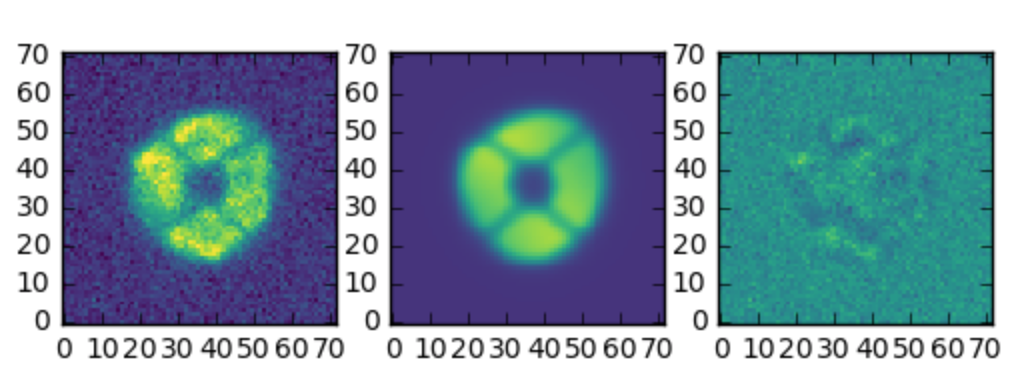
\includegraphics[width=0.5\textwidth]{figures/donut.png}\\
  \tiny Figure: Meyers, \citeds{DMTN-064}
  \end{center}
}

\end{frame}

\begin{frame}{Data Release Production}

\textbf{And more!}
\begin{itemize}

  \item{Work getting started on:

    \begin{itemize}

      \item{Star-galaxy separation}
      \item{New galaxy fitting algorithm}

    \end{itemize}

    ... watch for news at the LSST 2018 Joint Technical Meeting.}

    \item{Lots of effort going into Butler Generation 3.}

\end{itemize}

\end{frame}

\frame{\frametitle{Data Access Services}
\begin{columns}
    \begin{column}{0.6\textwidth}
        \begin{itemize}
            \item Catalog Database (Qserv) to 100 TB range
            \begin{itemize}
                \item Three 30-node clusters operating:
                \begin{itemize}
                    \item NCSA (PDAC): science dataset (Stripe 82 + AllWISE + NEOWISE)
                    \item CC-IN2P3 (2 x dev): synthetic dataset
                \end{itemize}
                \item 30\% DR1 KPM measurements in progress
                \item Jun 2018:
                    \begin{itemize}
                        \item Deployment under Kubernetes
                        \item Data replication and auto-recovery
                        \item Revamped loader/ingest tools
                        \item HSC load
                    \end{itemize}
                \item Dec 2018:
                    \begin{itemize}
                        \item Gaia DR2 load
                    \end{itemize}
            \end{itemize}
        \end{itemize}
    \end{column}
    \begin{column}{0.4\textwidth}
        \begin{center}
            \includegraphics[width=\columnwidth]{figures/qserv-in2p3.png}
        \end{center}
    \end{column}
\end{columns}
}

\frame{\frametitle{Data Access Services}
\begin{columns}
    \begin{column}{0.7\textwidth}
        \begin{itemize}
            \item Web Services for Science Platform -- Standards Orientation\\~
            \begin{itemize}
                \item Bespoke endpoints now being replaced with IVOA compliant services:
                    \begin{itemize}
                        \item TAP/ADQL, SIAv2, SODA, VOspace, UWS
                    \end{itemize}
                \item Standards-oriented metadata:
                    \begin{itemize}
                        \item RegTAP, VOResource, ObsCore, CAOM, UCD
                    \end{itemize}
                \item Jun 2018: Revamped TAP/ADQL query services
                \item Dec 2018: Revamped image cutout and metadata services
            \end{itemize}
        \end{itemize}
    \end{column}
    \begin{column}{.3\textwidth}
        \begin{center}
            
\includegraphics[width=\columnwidth]{figures/ivoa.jpg}
        \end{center}
    \end{column}
\end{columns}
}

\frame{\frametitle{Middleware}
\begin{itemize}
    \item Gen 3 Data Butler and Supertask\\~\

    An object-oriented data archive abstraction (Butler) and workflow infrastructure (Supertask).  Needed cleanup/attention!\\~\
    \begin{itemize}
        \item Working group convened; from scratch in-depth exploration of use cases
        \item New design resulted; scrum team assembled
        \item Jun 2018: support for HSC camera
        \item Dec 2018: replace Gen 2 code throughout DM stack
    \end{itemize}
\end{itemize}
}

\frame[allowframebreaks]{\frametitle{LSST Data Facility (NCSA)}

\begin{itemize}
\item  Observatory Operations Support (Level 1) Services

\begin{itemize}
\item Working closely within the LSST Systems Engineering Early Pathfinder group, developing and incrementally testing integration of T\&S, Camera, and DM service software via a series of early integration activities.
    \item Initial header service developed and configured for Camera subsystem and AuxTel use cases, ability to acquire pixel data and write FITS files, all commandable by OCS. Demonstrated on Level 1 Complete Test Stand.

\end{itemize}
\item Offline Campaign Processing and Batch Production Services

\begin{itemize}
    \item Production processing of HSC data for 503-2 milestone, working with DRP group.
    \item Upgrades to existing production framework based on DES data management system, including migration to Python 3.
    \item Continued regular dataset reprocessing to provide datasets for developers based on biweekly stack updates.

\end{itemize}
\item Data Backbone Services

\begin{itemize}
    \item Single-node consolidated database operational, supporting integration and testing of the batch production service.
    \item Provided operations use cases and developed requirements for Gen3 middleware working groups.

\end{itemize}
\item Container Application Management Services

\begin{itemize}
    \item Investigated deployment documentation and service level configurations requirements for FY18 Kubernetes deployment.
    \item Worked with SLAC, SQuaRE, and IPAC for requirement investigation and deployment configurations for initial use case support.

\end{itemize}
\item Developer Support Services

\begin{itemize}
    \item Upgrades to PDAC, including new dedicated Qserv head node provisioned in PDAC and interim Kubernetes installed on single PDAC node for special testing
    \item LSST-DB (MySQL developer database) replacement provisioned.
    \item Expand Level 1 Complete Test Stand to support early pathfinder testing and other cross-subsystem use cases.

	\end{itemize}
\item ITC and Facility

	\begin{itemize}
    \item 11 of 18 FY17 and FY18 capabilities provisioned including: initial production Kubernetes cluster, infrastructure for Chilean Base network security and identity management endpoint (shipped, installed, tested, and shipped), 3PB GPFS expansion for initial production file systems, consolidated database (Oracle cluster), Level 1 Complete Test Stand expansion, system for Tucson ATS Test Stand, data transfer nodes, disaster recovery capability for site file systems, central core network upgrade supporting large capability expansion.
    \item Matured system configuration management and operations with xCAT and Puppet.

	\end{itemize}
\includegraphics[width=0.8\textwidth]{NCSA-2018}

\item Service Monitoring and Management

\begin{itemize}
    \item LDF service monitoring framework designed, implemented, and deployed; beginning integration of systems and base services.

\end{itemize}
\item Other technical work within the project

	\begin{itemize}
    \item Lossy Compression Working Group
    \item Data Access Working Group -- policies at the project-level
    \item End-to-end long-haul network test
	\end{itemize}
\end{itemize}
}


\frame{\frametitle{NCSA - 2018 plans }
\begin{itemize}
\item  AuxTel Operations (Fall) (LSST- and DM-level milestones)

	\begin{itemize}
    \item AuxTel Test Stand operations (April).
    \item Provisioning of Chilean ITC (Summit facility) for AuxTel operations.
    \item Spectrograph Archiving Service building raw images, Header Service.
    \item Data transfer to NCSA, ingestion and archiving into initial version of production Data Backbone (single site).
    \item CPP production processing.
    \item EFD ETL Service operational, including database and Large File Annex.
	\end{itemize}
\item Chilean Base AA and security monitoring systems installed, services deployed, and monitored (April 2018) in NOAO facility.
\item Application-level integration with service monitoring framework, initial  dashboards for service operations and capacity management
\item Supporting ongoing development

	\begin{itemize}
    \item Initial Kubernetes Service in VERY friendly user mode March 2018. Integration for developers use cases (e.g., hosting Jupyter notebooks, Alert Distribution system testing, etc.) throughout CY18.
    \item Full HSC PDR reprocessing campaign and continued dataset processing.
    \item Continue providing production-oriented input into Gen3 Middleware development, including design, testing, and planning use in production framework.
    \item Improvements to Developers Support Services.
	\end{itemize}
\end{itemize}
}


\frame{\frametitle{Base \& Network}

\begin{itemize}
\item The Network Engineering Team completed the first successful transfer of digital data over LSST/AURA fiber optic networks from the Summit Site on Cerro Pachon to the Base Site in La Serena and on to the Archive Site at NCSA in Champaign. A set of 6 x 10 Gbps Network Interface cards on Data Transfer Nodes (DTN) configured with iPerf3 generated a sustained data rate of approximately 44 gigabits per second, over a period of 24 hours, exceeding the target of 40 gigabits per second.

\end{itemize}
}

\frame{\frametitle{SQuaRE}
\begin{columns}
    \begin{column}{0.6\textwidth}
        \begin{itemize}
            \item Current status and recent highlights:
            \begin{itemize}
                \item Notebook Aspect meets most requirements. Deployments:
                \begin{itemize}
                    \item Two SQuaRE development deploys on GKE (1 stage, 1 semi-prod)
                    \item Other deploys: SysEng, EPO, tutorials
                    \item DM deploy coming soon on LDF k8 commons prototype
                \end{itemize}
                \item CI developer wishlist done including much improved Slack notifications
                \item SQuaSH 
                    \begin{itemize}
                        \item Developer metric support in pre-release testing
                        \item Replaced Django with flask to match other teams technical stack
                        \item Moved architecture to Kubernetes for consistent deployment in LDF
                    \end{itemize}
                \item Documentation:
                    \begin{itemize}
                        \item lsst.io landing page / doc index
                        \item Pipelines getting-started tutorial
                        \item package documentation example using `pipe_base`
                        \item LaTex support for LSST-The-Docs
                    \end{itemize}
            \end{itemize}
        \end{itemize}
    \end{column}
    \begin{column}{0.4\textwidth}
        \begin{center}
%            \includegraphics[width=\columnwidth]{qserv-in2p3.png}
        \end{center}
    \end{column}
\end{columns}
}

\frame{\frametitle{SUIT: Major Achievements}

\begin{itemize}
   \item{New Features in PDAC}
      \begin{itemize}
         \item{Search and display WISE single epoch sources}
         \item{Incorporated the DAX imgServ v1 in SUIT}
      \end{itemize}
   \item{Visualization}
      \begin{itemize}
         \item{Search and display HiPS images}
         \item{Multiple scattered plots within one plotting area }
      \end{itemize}
   \item{Build and deployment}
      \begin{itemize}
         \item{Experimented with docker and Kubernetes}
         \item{Added Jenkins task to build Firefly docker image}
         \item{Added Jenkins tasks to deploy/destroy Firefly application as Kubernetes pod}
      \end{itemize}
   \item{Implemented embedded database HyperSQL for table data support in Firefly}
   \item{Updated 3rd party packages: React, Webpack ...}
   \item{Various improvements  and bug fixes}
\end{itemize}
}

\frame{\frametitle{SDSS HiPS images in Firefly}
\vspace{-10pt}
\begin{center}
 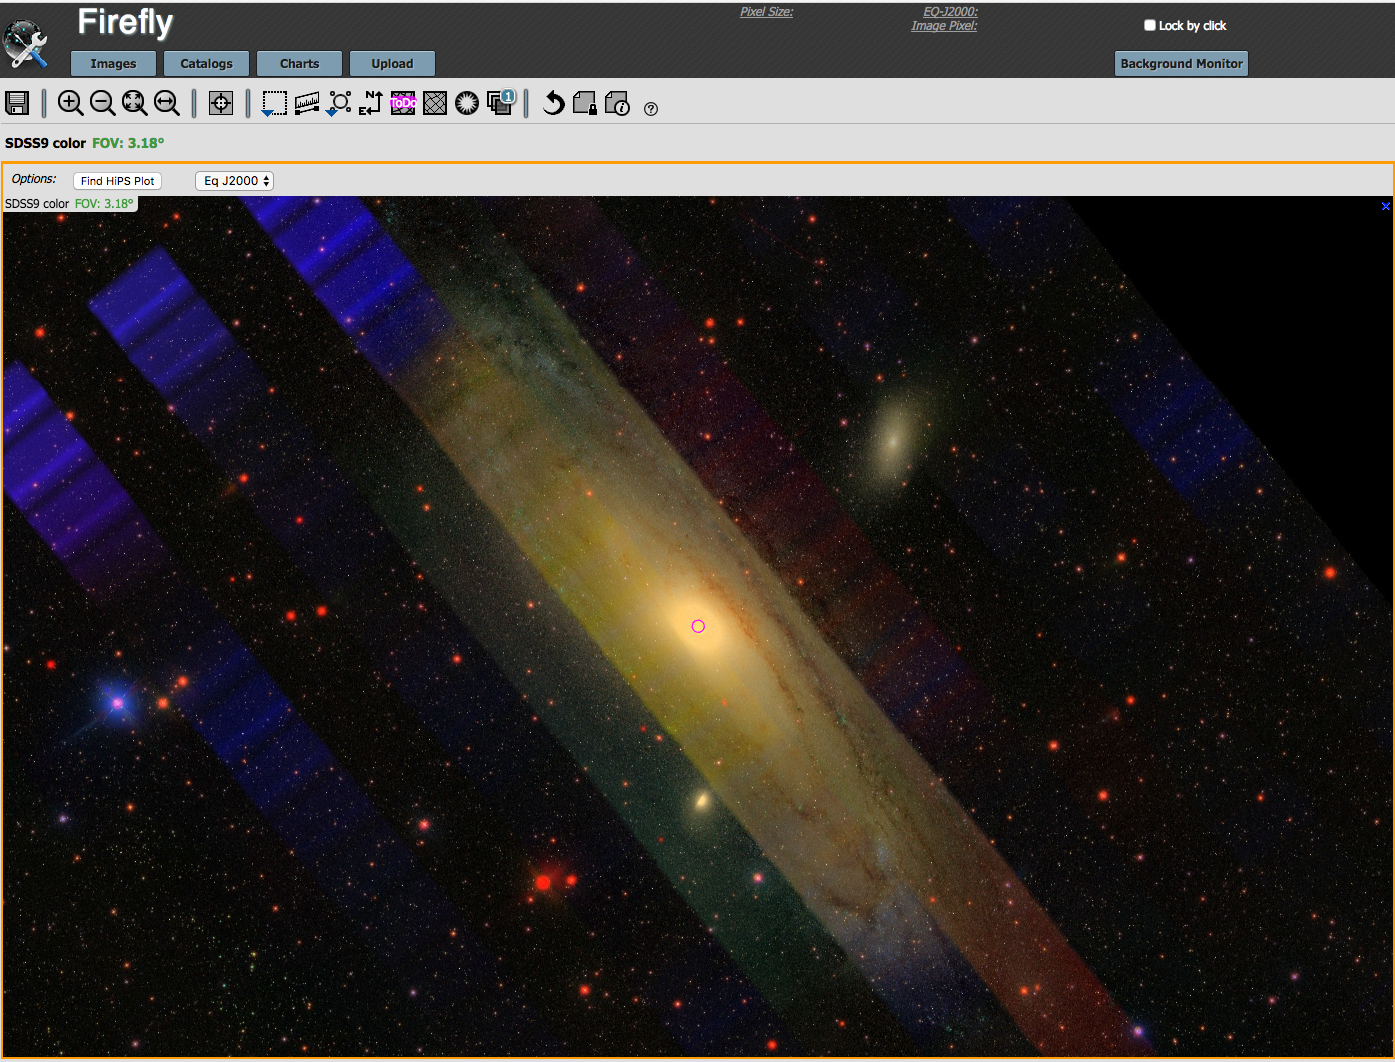
\includegraphics[width=0.7\textwidth]{sdssM31HEALPix1.png}
 \end{center}
}
\frame{\frametitle{SUIT: Plan for Next 6 Months}
\begin{itemize}
   \item{New Features in PDAC}
      \begin{itemize}
         \item {Search and display HSC data reprocessed by LSST pipeline}
         \item {Use the new version of DAX APIs: metaServ, imgServ, dbServ}
         \item {Integrate the authentication system}
         \item {Access workspace when available}
      \end{itemize}
   \item {Improve overall user experience in SUIT}
   \item {Make Firefly npm installable to support using Firefly API in JupyterLab}

\end{itemize}

}


\frame{\frametitle{Subsystem Science Team (SST)}

\begin{itemize}
\item Data Access Policy LSE-349 draft prepared; now under review by project management
\item Alerts Broker Policy LDM-612 draft is underway; UW broker team focused on ZTF Alerts
\item DM & Special Programs DMTN-065 spawned RFC-412 and Jira tickets under discussion (to close in next ~month)

\end{itemize}
}
\section{Conclusion}

\frame{\frametitle{Conclusion}
\begin{itemize}
\item New DM Project Management almost 1 year on the job !
\item We had a successful NSF/DOE Review in July 2017.
\item Will need to show verification for this summer
\item We move to implementation less experimentation - need to get things working
\item Starting  with AuxTel !
\item Thank you all for your continued efforts!

\end{itemize}
}

\frame {
  \frametitle{ The END }
\vspace{-0.3cm}
\begin{center}
 \includegraphics[width=0.4\textwidth]{images/SDSScosmos}
\hfill
 \includegraphics[width=0.4\textwidth]{images/HSCcosmos}\\
\vspace{-3.2cm}\hspace{0.7cm} \huge{\color{red} Questions?}\\
\vspace{+2.2cm}
\normalsize
{$\sim  3.5 \arcmin$ SDSS image   \hfill  HSC image (COSMOS)   \\\hfill \tiny g,r(1.5 hrs) ,i(3 hrs) PSF matched co-add ($\approx 27.5$)\\}

\vspace{-5pt}
{\tiny \url{http://www.lsst.org}} {\tiny \url{http://community.lsst.org}} \hfill
{\tiny Images:Lupton and HSC colaboration see also \cite{2004PASP..116..133L}}
\end{center}

}




\appendix

\section {Reference material}
\frame[allowframebreaks]{\frametitle{ Acronyms }
        \vspace{10pt}
        \tiny
        \addtocounter{table}{-1}
\begin{longtable}{|l|p{0.8\textwidth}|}\hline
\textbf{Acronym} & \textbf{Description}  \\\hline

AURA&Association of Universities for Research in Astronomy \\\hline
C&Specific programming language (also called ANSI-C) \\\hline
DM&Data Management \\\hline
ESA&European Space Agency \\\hline
ESAC&European Space Astronomy Centre (VilSpa) \\\hline
ESOC&European Space Operations Centre (ESA) \\\hline
ESTEC&European Space research and TEchnology Centre (ESA) \\\hline
HEALPix&Hierarchical Equal-Area iso-Latitude Pixelisation \\\hline
HTM&Hierarchical Triangular Mesh \\\hline
LSST&Large Synoptic Survey Telescope \\\hline
PhD&Doctorate in Philosophy \\\hline
SDSS&Sloan Digital Sky Survey \\\hline
TEC&Thermo-Electric Cooler \\\hline
USA&United States of America \\\hline
arcmin&arcminute, minute of arc (unit of angle) \\\hline
arcsec&arcsecond, second of arc (unit of angle) \\\hline
\end{longtable}

}

\frame[allowframebreaks]{\frametitle{ References }
       \tiny
       \bibliographystyle{lsst_aa}
       \bibliography{lsst,gaia_livelink_valid,refs,books,refs_ads}
       \normalsize

}



\end{document}
